\documentclass[conference]{IEEEtran}

%XXX Remove before final submission
\usepackage{todonotes}
\usepackage{cite}
\usepackage{amsmath}
\usepackage{caption}
\usepackage{subcaption}
% Note that the amsmath package sets \interdisplaylinepenalty to 10000
% thus preventing page breaks from occurring within multiline equations. Use:
%\interdisplaylinepenalty=2500
% after loading amsmath to restore such page breaks as IEEEtran.cls normally
\usepackage{url}
\usepackage{hyperref}
\usepackage{verbatim}
\usepackage{listings}

\lstdefinelanguage{Julia}{
  basicstyle=\small\ttfamily,
  showspaces=false,
  showstringspaces=false,
  keywordstyle={\textbf},
  morekeywords={if,else,elseif,while,for,begin,end,quote,try,catch,return,local,abstract,function,stagedfunction,macro,ccall,finally,typealias,break,continue,type,global,module,using,import,export,const,let,bitstype,do,in,baremodule,importall,immutable},
  escapeinside={~}{~},
  morecomment=[l]{\#},
%  commentstyle=\textsf,
  commentstyle={},
  morestring=[b]",
}

\lstset{language=Julia,basicstyle=\footnotesize\ttfamily,breaklines=true}

% correct bad hyphenation here
\hyphenation{}


\begin{document}

%XXX remove before submission
\newcommand{\TODO}[1]{\todo[inline]{#1}}
\newcommand{\TODOFIG}[1]{\missingfigure{#1}}

\title{Which Program Is Slower? Hypothesis Testing for Performance Regressions}

% author names and affiliations
% use a multiple column layout for up to three different
% affiliations
\author{\IEEEauthorblockN{Jiahao Chen and Jarrett Revels}
\IEEEauthorblockA{Computer Science and Artificial Intelligence Laboratory\\
Massachusetts Institute of Technology\\
Cambridge, Massachusetts 02139--4307\\
Email: \{jiahao,jrevels\}@csail.mit.edu}
}

% make the title area
\maketitle

%%%%%%%%%%%%%%%%%%%%%%%%%%%%%%%%%%%%%%%%%%%%%%%%%%%%%%%%%%%%%%%%%%%%%%%%%%%%%%%%%%%%%%%%%%%%
\begin{abstract}
We propose a rigorous methodology for automated microbenchmarking and regression detection
in the presence of timer error, OS jitter and other environmental fluctuations. By examining
data obtained from Julia microbenchmarks, we demonstrate the ways in which timing
distributions can violate many of the statistical assumptions made by other benchmarking
frameworks. From our experimental observations, we construct a model and an accompanying
microbenchmarking strategy which purposefully avoids these assumptions. This strategy makes
efficient use of user time constraints by simultaneously maximizing the number of
measurements per trial while minimizing inter-measurement timing variations, rendering it
suitable for continuous integration (CI) pipelines, even when applied to relatively large
benchmark suites. Using our model, we formulate a robust, nonparametric hypothesis test that
makes use of the bootstrap resampling method to estimate the statistical significance of
observed variations in execution time. We test our methodology on a small collection of mock
Julia benchmarks, discussing where it succeeds relative to other methods as well as pointing
out potential pitfalls. Finally, we discuss a prototype implementation of the proposed
method that was recently released to aid in the development of the Julia language and
ecosystem, which has already caught and prevented several performance regressions in Julia's
base library.
\end{abstract}

\IEEEpeerreviewmaketitle

%%%%%%%%%%%%%%%%%%%%%%%%%%%%%%%%%%%%%%%%%%%%%%%%%%%%%%%%%%%%%%%%%%%%%%%%%%%%%%%%%%%%%%%%%%%%
\begin{comment}
    The myraid sources of environmental variation must all be mitigated against to
    produce a reproducible state in which to run the benchmark program. In practice,
    it is impossible to eliminate variation entirely~\cite{Alcocer2015,Barrett2016}.
    Therefore, it is still necessary to think about statistics.

    A common assumption is that it suffices to ``warm up'' the machine by running the
    benchmark program a few times, after which the becnhmarks will run at peak performance.
    On the contrary, practically no benchmarks exhibit such simplistic behavior. Studies of
    statistics of repeated benchmarks agree that the distributions observed in practice are
    highly nonnormal and have large outliers. Some benchmarks even exhibit correlation
    between consecutive timing measurements.

    Some examples of these behaviors can be seen in Figure~\ref{fig:examplebenchmarks}, even
    for the very simple benchmarks that we describe in this paper. As a result, simple
    textbook statistical tests like $t$-tests and $F$-ratios, which assume iid normality,
    have poor statistical power, as discussed
    in~\cite{Mytkowicz2009,Kalibera2013,Chen2015,Barrett2016}. There have been several
    approaches to this problem.

    The first approach is to remove outliers~\cite{Rehn2015}\TODO{and loc. cit.} to improve
    Gaussianity. However, it is unclear whether automated outlier removal can restore the
    ability to use Gaussian statistics for these benchmarks without introducing significant
    bias, particularly when the timing distributions are bimodal or multimodal.

    The second approach is to use biased variances to correct for
    non-Gaussianity~\cite{Mytkowicz2009}\TODO{check citation}. However, these corrections
    inherently assume that the statistics are close to Gaussian, and so there will be
    benchmarks for which this approach may fail to correct for non-Gaussianity.

    A third approach is to use robust statistics such as the median as a location
    parameter~\cite{Mytkowicz2009}, the interquartile range as a dispersion
    parameter~\cite{Mytkowicz2009}, or the medcouple for measuring skewness~\cite{Rehn2015}.
    The approach we propose here is most similar to this category of analyses, but we focus
    on the minimum instead.

    An additional consideration for microbenchmarks (benchmarks with very short execution times)
    is the measurement accuracy provided by the system timer.
    Taking one timing measurement of many executions reduces the measurement error,
    much as how the weight of a single sheet of paper can be measured more accurately
    by weighing 500 sheets at once and dividing the measurement by 500,
    as compared with weighing just one sheet directly.
    However, the longer the total run time of a timing measurement, the more likely
    the benchmarking process will incur environmental fluctuations.
    Therefore, commonly used rules of thumb like
    ``repeat the benchmark as many times as necessary so that the timing measurement
    is at least 5 seconds'' may not produce the most accurate estimate for the
    execution time of a microbenchmark.

    There is also some work on software tools for the statistical analysis of benchmarks.
    The Speedup-Test is an R package for analysing benchmark data~\cite{Touati2013}.
    There is also the framework of Chen et al 2015~\cite{Chen2015}.
    \TODO{Jarrett has more}


    In this paper, we present a fully automated framework for benchmarking that
    combines and extends the best practices noted by previous authors.

    \begin{itemize}
    \item
    We present a statistical model explaining why for the most part, fluctuations
    in timing measurements due to enviromental factors are always positive.
    Therefore, the minimum timing measurement produces the best estimate for
    the true execution time of a benchmark when the relative error incurred by
    system timer accuracy is negligible.

    \item
    For microbenchmarks, we formulate a search for the optimal number of evaluations
    a benchmark should be run for each timing measurment, striking a balance between
    the error incurred by timer inaccuracy and the delays accrued by environmental
    factors. For regression testing, it is only necessary to perform the search once
    per benchmark, and we regard the search is a preprocessing step to be performed
    separately from the collection of timing measurements used for testing for
    performance regressions.

    \item
    We formulate the statistical question of whether a program introduces a performance
    regression relative to another program as a hypothesis test. We propose the
    ratio of observed minima as a test statistic, which is robust to large outliers
    and is well defined for the distributions we expect from our statistical model.
    \end{itemize}

    We demonstrate that our approach works well for a collection of sample Julia
    benchmarks, correctly detecting regressions with low misclassification rates.
\end{comment}

%%%%%%%%%%%%%%%%%%%%%%%%%%%%%%%%%%%%%%%%%%%%%%%%%%%%%%%%%%%%%%%%%%%%%%%%%%%%%%%%%%%%%%%%%%%%
\label{sec:stats}
\section{A statistical interpretation of our microbenchmark results}

\begin{comment}
    We only focus on stateless benchmarks $P_0$, so that in principle, the benchmark program
    can be run many times, each time producing the same deterministic output. Even though
    the benchmark program $P_0$ itself may be stateless, its environment---the hardware it
    runs on, the operating system, and other programs that may also be running on the
    machine, for example---does carry some state and produces side effects which introduce
    variations in the runtime of $P_0$.

    In order to classify regressions in the presence of these variations, we need to develop
    a rigorous statistical model for our runtime that incorporates them.

    \subsection{Definitions and notation}

    There are several kinds of variables we use that have dimensions of time, and for
    clarity we define all of them here.

    A \textbf{benchmark execution time} $t$ is the smallest time scale, referring to how
    long it takes to execute the benchmark once. We normally do not time single executions
    directly.

    A \textbf{timing measurement} $T_i$ is the smallest experimentally measured quantity,
    consisting of multiple executions $n_i$ of the benchmark. The subscript $i$ labels each
    timing. From each timing measurement we can derive an indirect measurement of $t_i =
    T_i/n_i$.

    A \textbf{trial} is the largest grouping of time, referring to a collection of timing
    measurements. When we talk about multiple trials, $k_{\textrm{trials}}$ is the number of
    trials and each trial is indexed by an embraced subscript, $\cdot^{\{i\}}$. The $i$th
    trial has $k^{\{i\}}$ timings, and $T^{\{i\}}_j$ is the $j$th timing in the $i$th trial.

    To specify the linear search strategy in Section~\ref{sec:linearsearch}, we require
    $\tau_{\textrm{budget}}$, a time budget to do the linear search, $\tau_{\textrm{acc}}$,
    the accuracy of the system timer, and $\tau_{\textrm{prec}}$, the precision of the
    system timer.

    A \textbf{program} is composed of a series of \textbf{instructions}. $P_0$, $P$ and $Q$
    denote programs that we want to run as benchmarks. $I^{[i]}_{P_0}$ is the $i$th
    instruction in program $P_0$, where each instruction is indexed by a bracketed
    superscript, $\cdot^{[i]}$. $D^{[i]}_{P}$ is a delay instruction, which we define
    precisely in Section~\ref{sec:statmodel}.

    $\tau^{(i)}$ is a time scale associated with a \textbf{noise factor}, as defined below.
    Noise factors are indexed by parenthesized superscripts, $\cdot^{(i)}$.

    $x^{(i)[j]}$ is the number of times noise factor $i$ was triggered in delay instruction
    $j$. $X_P^{(i)}$ is the total number of times noise factor $i$ was triggered in running
    the program $P$.

    $\epsilon$ is a \textbf{measurement error} and has units of time.

    $\epsilon^{(i)[j]} = x^{(i)[j]} \tau^{(i)}$ is the time delay caused by noise factor $i$
    in instruction $j$. $E_P^{(i)}$ is the total cumulative time delay caused by noise
    factor $i$ over the course of running the program $P$.

    $\nu(t)$ is an oracle function which, given a time estimate, returns the number of
    executions per measurement.

    $f_X(\xi)$ is the probability density function (pdf) associated with the random variable
    $X$. $\int_{x}^{x+\delta x} f_X(\xi) d\xi$ is the probability that $x < X < x+\delta x$.

    \textbf{Estimated quantities} are denoted with a hat, $\hat\cdot$. For example, $\hat
    t_{min}$ is the estimated value for the minimum value of the benchmark execution time.

    \textbf{Resampled quantities} are denoted with a superscript asterisk, $\cdot^*$. For
    example, $t^*_1, \dots t^*_m$ is a resample of $t_1, \dots t_n$.
\end{comment}

\label{sec:model}
\subsection{A microscopic model for timing variations}

\begin{comment}
    The statistics we present can be justified with a simple microscopic model of program
    execution on a computer. Assume that we have only a single instruction pipeline and that
    the user's program $P_0$ may be specified as a single sequence of instructions
    $I^{[i]}$, which we shall denote by

    $P_0$ = \begin{tabular}{|c|c|c|c|c|}
    \hline
    $I^{[1]}$ & $I^{[2]}$ & $\dots$ & $I^{[N]}$ \tabularnewline
    \hline
    \end{tabular}.

    Assume that each instruction $I^{[i]}$ takes exactly time $\tau^{[i]}$ to execute. In an
    idealized universe, the user program $P_0$ will execute in time $t_{P_0} = \sum_{i=1}^N
    \tau^{[i]}$. However, in between any two consecutive instructions $I^{[i]}$ and
    $I^{[i+1]}$, the computer may choose to run zero or more instructions that are
    \textit{not} specified by the user program $P_0$. In effect, the computer has
    transformed the input program $P_0$ into a new program $P$, which interleaves the input
    sequence of instructions $I^{[i]}$ with delay instructions $D^{[i]}$:

    $P$ = \begin{tabular}{|c|c|c|c|c|c|c|c|c|c|}
    \hline
    $D^{[1]}$ & $I^{[1]}$ & $D^{[2]}$ & $I^{[2]}$ &
    $\cdots$ & $D^{[N]}$ & $I^{[N]}$
    \tabularnewline
    \hline
    \end{tabular}.

    The delay instructions $D^{[i]}$ model fluctuations arising from environmental triggers
    described in Section~\label{ref:intro} such as cache thrashing, thread scheduling or
    even network interrupts. The semantics of $P_0$ and $P$ are identical, but $P$ run takes
    time $t_P = t_{P_0} + \sum_{j=1}^N D^{[j]} > t_{P_0}$ to run.

    We can further decompose Further imagine that this machine has $N_f$ independent noise
    factors, which we label in superscripts $\cdot^{(i)}$. Each noise factor can trigger
    with probability $p^{(i)}$, and each time the noise factor is triggered, it will take
    time $\tau^{(i)}$ to run. Let $x^{(i)[j]} \in \{0, 1\}$ indicate whether the $i$th
    jitter factor is triggered each time in the random delay instruction $D^{[j]}$. Then the
    run time of $D^{[j]}$ is $\tau_{D^{[j]}} = \sum_{i=1}^{N_f} x^{(i)}_j \tau^{(i)}$ and is
    no longer deterministic, but instead a random variable.

    Putting all these things together, we get

    \begin{equation}
    t_P = t_{P_0} + \sum_{j=1}^N \sum_{i=1}^{N_f} x^{(i)[j]} \tau^{(i)}
    = t_{P_0} + \sum_{i=1}^{N_f} X_P^{(i)} \tau^{(i)},
    \end{equation}
    %
    where $X_P^{(i)} = \sum_{j=1}^N x^{(i)[j]}$ is the number of times the noise factor $i$
    was triggered when running the program $P$.

    The randomness has a natural interpretation in the Kolmogorov formulation of
    probability. We could in principle gather so much information about the exact
    microscopic configuration $\mathcal S$ of a computer, down to its precise hardware
    specification, operating temperature, and all the bits in its I/O streams, caches,
    buffers, and storage devices, and so on, that we could know deterministically how long
    each delay instruction $D^{[j]}$ would take to run. If we could also restore the
    computer to the precise state $\mathcal S$ after running the program $P$, then the
    computer will execute $P$ again with exactly the same, deterministic run time. In
    practice, however, we never know $\mathcal S$ with enough detail to describe $t_P$
    deterministically. Instead, we must make do with an imprecise specification of the
    machine state, saying instead that the machine state $\mathcal S$ is only known to
    belong to some set $S$ of possible machine states belonging to the sample space
    $\Omega$. In this sense, our probabilistic description of program execution is
    reminiscent of the microcanonical ensemble in statistical mechanics.

    Let's note a few properties of this model:

    First of all, $t_P \ge t_{P_0}$ since each characteristic time $\tau^{(i)} > 0$ is
    positive. Therefore $P$ always takes more time to execute than $P_0$. For this model to
    apply, we must assume that jitter that causes \textit{faster} execution times, such as
    frequency boosting, are absent and disabled with the appropriate hardware and OS
    configuration settings~\cite{benchmarktoolschecklist}. We have equality $T_P = T_{P_0}$
    for machine states $\mathcal S_0$ that trigger no jitter whatsoever. Such a machine
    state may not exist, but nevertheless there must exist some state (or collection of
    states) $\mathcal S_<$ that minimizes $t_P$ to some value, $t_{<P}$, invoking the fewest
    possible jitter factors that lead to smallest possible increase in execution time over
    $t_{P_0}$. Statistically speaking, there must exist some critical time $t_{<P}$ for
    which the probability density function (pdf) $f_{t_P}(\xi)$ of $t_P$ of obeys
    $f_{t_P}(\xi) = 0 \; \forall \; \xi < t_{<P}$.

    Secondly, there are special case limiting behaviors that make a lot of sense. For
    example, if there is only $N_f = 1$ factor of OS jitter, then $X^{(1)}$ follows a
    binomial distribution with $N$ samples and proability $p^{(1)}$. If furthermore the
    number of instructions $N$ is sufficiently large, then and there is only $N_f = 1$
    factor of OS jitter, then the behavior of $X^{(1)}$ follows a Poisson (exponential)
    distribution with rate $p^{(1)} N$.\TODO{Fix description of ideal behavior - Andreas
    points out it's not right} If there are $N_f > 1$ factors of OS jitter, each with
    identical trigger probability $p^{(i)} = \pi$ and characteristic time scale $\tau^{(i)} =
    \tau$, then $X = \sum_{i=1}^{N_f} X^{(i)}$ follows an Erlang distribution with shape
    parameter $k$ and rate $p^{(1)} N$. Of course in practice, few benchmarks obey such
    idealized behavior, but they are useful limiting cases to bear in mind. Furthermore our
    model is general enough to cover the wide variety of distributions seen in practice. An
    important nonideal case is the observation of two or more modes in $f_{t_P}$. Such
    behavior is consistent with a model $t_P = t_Y Y + t_Z Z$, where $t_Y$ and $t_Z \ne t_Y$
    are constants describing a characteristic time scales associated with random variables
    $Y$ and $Z$ respectively, and $Y$ is an Erlang distribution and $Z$ is a binomial
    distribution.

    \TODO{Do we ever recover Gaussianity?}
\end{comment}

%%%%%%%%%%%%%%%%%%%%%%%%%%%%%%%%%%%%%%%%%%%%%%%%%%%%%%%%%%%%%%%%%%%%%%%%%%%%%%%%%%%%%%%%%%%%
\label{sec:protocol}
\section{Protocol for experiment configuration and benchmark execution}

\begin{comment}
    For benchmarks that take very little time to run, it is vital to run it many times so
    that you avoid measurement error coming from finite timer accuracy. We distinguish
    between precision and accuracy here: just because the system may provide a timer with
    nanosecond precision does not automatically guarantee that it has nanosecond
    \textit{accuracy}. In principle we can calibrate the timer for a given system to measure
    its accuracy. In practice, we simply assume a given accuracy, say 1 microsecond, and
    proceed accordingly.

    A common rule of thumb used in practice is to repeat the benchmark enough times, say
    $n$, so that the total execution time exceeds a certain minimum period, say 5--20
    seconds. The relative accuracy of assessing the actual run time is increased. A useful
    analogy is how you can get a more precise measurement of the weight of a single sheet of
    paper if you weigh 500 sheets on scale and divide the measurement by 500, as opposed to
    weighing just a single sheet directly.

    Nominally it looks like the relative accuracy of this process should be 1 μs/10s =
    $10^{-7}$. However, the longer you run the program the more OS jitter you will pick up
    in the timing. Different benchmarks pick up different jitter. For example memory heavy
    benchmarks may pick up more cache misses while I/O heavy benchmarks may pick up more
    hard disk latency. So in practice you want to run the benchmark long enough to minimize
    timer accuracy error while not pick up too much jitter, and a hard rule of thumb like
    5--20 seconds may be too much or not enough.

    Some benchmarking libraries, like Haskell's criterion~\cite{criterion}, advocate a
    linear search methodology to choose the optimal $n$ where you keep increasing the number
    of repetitions linearly up to a fixed upper bound, say 1 minute, then do a linear
    regression to find which region starts to exhibit linear scaling with the number of
    repetitions. However, a common error in these descriptions is that they tend to also
    include many data points with total times comparable or less than the timer accuracy.
    Actually we should throw all of these away because having many inaccurate points biases
    the least squares search. Or maybe we should do instead weighted least squares so that
    the regression knows something about error bars. In practice throwing away the short
    runs suffices. Also you don't want to have too many data points with very long run times
    because you may start to trigger new jitter factors with longer characteristic time
    scales.

    Let's justify the linear search strategy. Let $h$ be the timer accuracy, $n_1, n_2, ...,
    n_k$ be a sequence for the number of repetitions $n$ to be tried, and $T_j$ be the
    execution time measured when the number of repetitions is $n_j$. We assume that the
    measured execution time can be decomposed into

    \begin{equation}
        \label{eq:linsearch}
        T_j(n_j) = n_j \tau_{true} + \epsilon + \sum_{i=1}^{N_f} X_j^{(i)} \tau^{(i)}
    \end{equation}

    where $\tau_{true}$ is the true benchmark execution time. If the last two terms are
    constant then a linear regression will have slope $\tau_{true}$ and intercept $\epsilon +
    \sum_{i=1}^{N_f} X_j^{(i)} \tau^{(i)}$. But $\epsilon$ is not deterministic.
    Furthermore, the jitter term will also grow with $n_j$ and this complicates the
    analysis. However, if we assume that $\epsilon$ is independent of $n_j$ and that each
    $X_j^{(i)} = O(n_j)$, then by definition, there then exist positive constants $M^{(i)} >
    0$ such that for all sufficiently large $n_j$, $X_j^{(i)} < M^{(i)} n_j$, in which case
    the observed gradient is $\tau_{obs} = \tau_{true} + \sum_i M^{(i)} >
    \tau_{true}$\footnote{If we have instead that $X_j^{(i)} = o(n_j)$, then the gradient
    asympotitically is just $\tau_{true}$}.

    \begin{figure}
    \centering
    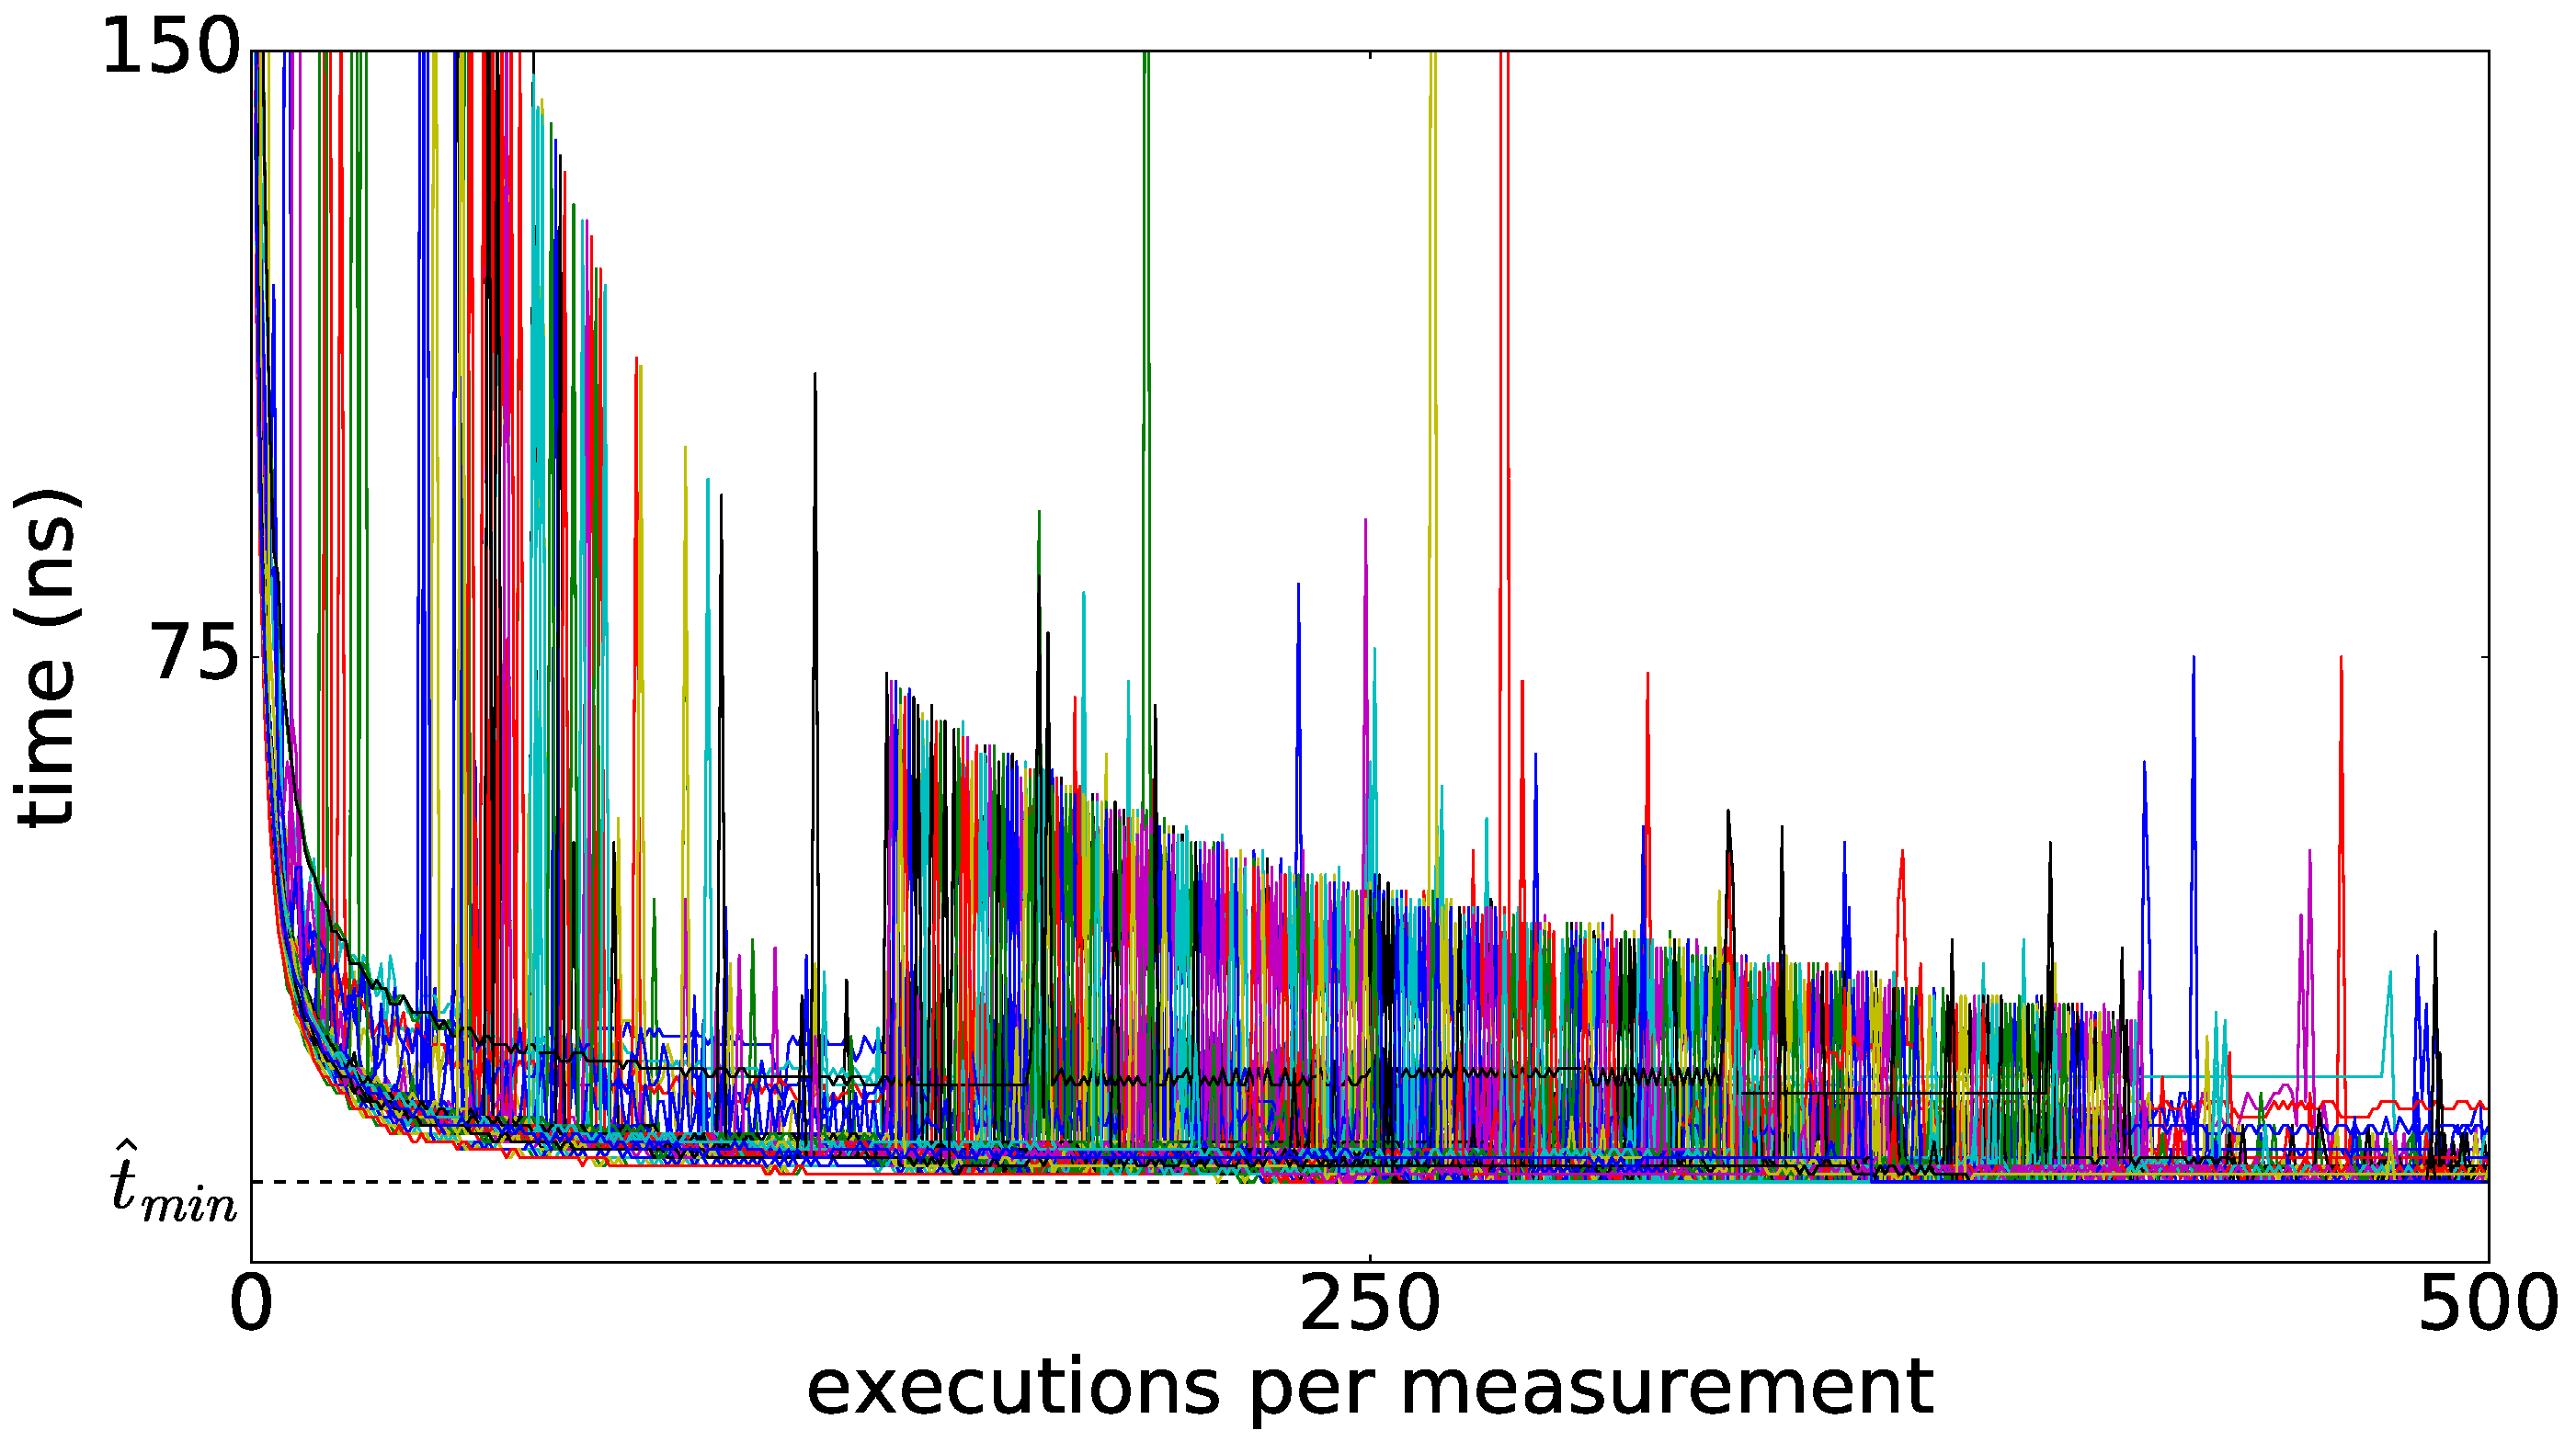
\includegraphics[width=0.45\textwidth]{figures/fig2/linear_scan_branchsum}
    \caption{$t_j = T_j(n)/n$ for many repeated linear scans for a particular benchmark,
             where $T_j$ is defined in \eqref{eq:linsearch}. Each curve denotes a different
             linear scan. Note the large spikes produced by jitter.}
    \label{fig:scaling}
    \end{figure}

    In practice, we observe that there are some benchmarks that pick up jitter factors with
    very large time scales. An example of such a benchmark is shown in Figure~These
    occurrences can be explained in several ways in our model. The simplest way is to posit
    some factor $l$ for which $\tau^{(l)} = O(n_j \tau_{true}) = O(n_j)$ and $X_j^{(i)}(n) =
    H(n - n^\ddagger)$, where $H$ is the Heaviside step function. The existence of such a
    factor produces a discontinuity in the gradient at $n^\ddagger$. In practice, some
    caution must be taken to avoid triggering such a jitter factor.

    We therefore recommend a truncated linear regression trimming all runs lasting less than
    the timer accuracy of 1 μs. \TODO{This is not the correct description of what we
    actually do}
\end{comment}

Given a benchmarkable program $P$ and a time budget $\tau_{budget}$, we'd like to define $n$, the number of executions of $P$ to perform for each timing measurement, such that a trial of our experiment...

\begin{itemize}
    \item ...produces timing estimates as close to the lower bound $t_{min}$ as possible
    \item ...minimizes the variance between timing estimates
    \item ...maximizes the number of timing measurements we are able to obtain under the constraint of $\tau_{budget}$
\end{itemize}

Given a timer accuracy $\tau_{acc}$ and a timer precision $\tau_{prec}$, our algorithm for tuning $n$ is as follows:

\begin{enumerate}
\item For $n \in \{1...\tau_{acc}\}$, measure the amount of time it takes to perform $n$ executions of $P$. The result of this step is a collection of timing measurements $T_n$ for all $n$.
\item From the derived timing estimates $t_i = T_i / i$, select the minimum timing estimate $\hat{t}_{min}$.
\item To obtain $n$, plug $\hat{t}_{min}$ into an oracle function $\nu(t_i) \to n_i$. Given $\tau_{acc}$ and $\tau_{prec}$, the properties of $\nu(t)$ are as follows:
\begin{itemize}
    \item $\nu(\tau_{prec}) \approx \tau_{acc}$
    \item $\nu(\tau_{acc}) \approx \text{small} (\sim 10)$
    \item $\nu(t \gg \tau_{acc}) \approx 1$
    \item $\frac{d\nu}{dt}\big|_{t \approx \tau_{prec}} = \text{close to zero}$
    \item free of discontinuities \TODO{how to say this correctly since the range is discretized}
\end{itemize}
\end{enumerate}

%%%%%%%%%%%%%%%%%%%%%%%%%%%%%%%%%%%%%%%%%%%%%%%%%%%%%%%%%%%%%%%%%%%%%%%%%%%%%%%%%%%%%%%%%%%%
\label{sec:regressions}
\section{Hypothesis tests for regression detection}

We are now ready to make use of all this probablisitic machinery to describe the statistics
of regression benchmarking. Suppose we have a reference program $P$ and a modified program
$Q$ which produce the same output when given identical inputs. We now want to know if $P$ is
slower than $Q$. Again in a perfectly deterministic universe where there are no OS jitter
factors or the starting machine state $\mathcal S$ known with great precision and can be
reproduced on demand, then we simply run $P$, time how long it takes, reset the machine back
to its starting state $\mathcal S$, and then run $Q$, noting how long it takes to run.
However $\mathcal S$ is never known exactly, and even if it were known, it's not clear if
$\mathcal S$ represents a ``typical'' machine configuration encountered in practice.

We are thus inexorably led to consider instead the statistical question of whether

\begin{equation}
\Delta t = t_Q - t_P
= (t_{<P} - t_{<Q}) + \sum_{i=1}^{N_f} (X^{(i)}_P - X^{(i)}_Q) \tau^{(i)}
\end{equation}
%
is statistically positive.

What we need to do now is to distinguish the constant factor $t_{<P} - t_{<Q}$, the part we
care about, from the second term, representing differences in noise triggers.

\TODO{... SKIP SOME STEPS ...}

\subsection{Choice of location parameter}

There is a question of what location parameter to use. One may want to use the means, but as
we all know the means are sensitive to large outliers. We see large outliers in the
benchmark data, which happens when some OS jitter factor with a very long delay is
triggered. Figure~\ref{fig:locationmeasures} show the various kinds of behavior different
location measures can exhibit.

\begin{figure}
\centering
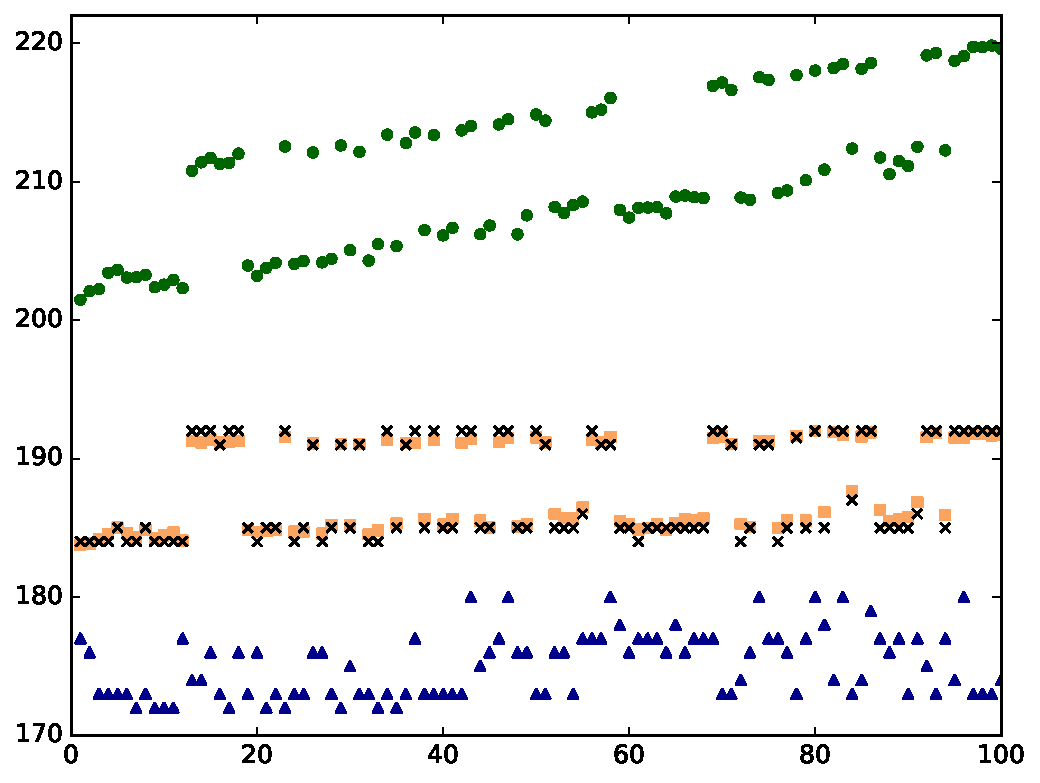
\includegraphics[width=\columnwidth]{figures/fig3/location_estimators_sumindex}
\caption{The behavior of different location parameters across multiple trials of
the \lstinline|sumindex| benchmark: mean (green filled circles), trimmed mean of
the 5th---95th percentiles (brown filled squares), medisn (black crosses), and
minimum (blue filled triangles).}
\label{fig:locationmeasures}
\end{figure}

Hypothesis testing based on location measures are sensitive to non-stationary OS jitter, for
example if there is some jitter factor $i$ such that $X^{(i)}_P = 1$ while $X^{(i)}_Q = 0$
determistically. There is a fundamental definition problem in this situation. If we
acknowledge that factor $i$ is always triggered once every time program $P$ runs but not in
$Q$, then we could could fold the contribution of factor $i$ into the definition of
$t_{<P}$, recognizing that it is not possible to run $P$ without triggering factor $i$.
However, it is impossible to distinguish statistically between this case and non-stationary
jitter, i.e.\ jitter that changes the machine's behavior for a time period longer than, say,
the combined run times of $P$ and $Q$. For example, the OS may decide to start paging
virtual memory to disk halfway through running $P$, which continues all throughout the time
when the user runs $Q$. Another possibility is that the machine running the benchmark
encounters an unusally high level of network traffic when running $P$ and $Q$, for example
if the machine is suffering a DDoS attack. The only way to detect this kind of nonstationary
noise is to run $P$ and $Q$ enough times so that the combined run time exceeds the
characteristic time scale for this jitter. However, in practice this may require benchmarks
to run for unacceptably long times.

It is easy to calculate the estimators $\hat d_P$ and $\hat d_Q$. However, we don't know
analytically what the distribution of $d_P - d_Q$ looks like, which we need to know in order
to describe the appropriate time scale $\tau$ to describe statistical significance. (This
time scale generalizes the standard error of the $t$-statistic when comparing the means of
two Gaussians.) So we use a bootstrap procedure to estimate this scale
$\tau$~\cite{Chernick2008}. The Julia code for the bootstrapping procedure for the test
statistic for $H_0$ vs.\ $H_1$ is

\begin{lstlisting}
"""
Resample test statistic z using m-of-n bootstrap

Inputs:
param   - function to compute location or dispersion
          parameter, e.g. mean, median, iqr
Ps, Qs  - sampled run times for programs P and Q
nresamp - size of resample
ntrials - number of resamplings
"""
function resamp(param, Ps, Qs, nresamp, ntrials)
    diff = zeros(ntrials)
    for i in 1:ntrials
        diff[i] = param(rand(Ps, nresamp)) -
                  param(rand(Qs, nresamp))
    end
    return diff
end

z  = median(Ps) - median(Qs)
zs = resamp(median, Ps, Qs, nresamp, ntrials)
p  = mean(z .> zs) #Compute p-value
\end{lstlisting}

\TODO{Say something about how we are doing m-of-n bootstrap, sampling without replacement,
and what are typical resample sizes and number of trials that give us reliable estimates.}

%%%%%%%%%%%%%%%%%%%%%%%%%%%%%%%%%%%%%%%%%%%%%%%%%%%%%%%%%%%%%%%%%%%%%%%%%%%%%%%%%%%%%%%%%%%%

\section{Implementation in Julia}

We have implemented the stastistical ideas described above in a suite of packages available
on GitHub under the \href{https://github.com/JuliaCI}{JuliaCI} organization. The code is
implemented in Julia. Julia is a programming language designed for technical computing, an
area where performance considerations are very important. The code is available freely on
GitHub under the MIT ``Expat'' License.

Some of this code we describe is also for ease of convenience for benchmarking the entire
Julia base library, which we do not discuss here.

\begin{itemize}
\item
\href{https://github.com/JuliaCI/BenchmarkTools.jl}{BenchmarkTools.jl} is a Julia package
for automated benchmarking and regression testing, implementing the statistical ideas
described above for automated regression testing. Its documentation also lists
\href{https://github.com/JuliaCI/BenchmarkTools.jl/blob/60dfe83e5434c87b7311ca5d9f185f45752ed510/doc/linuxtips.md}{recommendations
for improving quiescence and reducing timing variability}.
\item
\href{https://github.com/JuliaCI/BaseBenchmarks.jl}{BaseBenchmarks.jl} is a collection of
approximately 1,300 benchmarks which can be used for testing performance regressions in the
Julia base library and compiler.
\item
\href{https://github.com/JuliaCI/Nanosoldier.jl}{Nanosoldier.jl} contains GitHub API hooks
that trigger some or all the benchmarks to be run on the Nanosoldier, a dedicated machine at
MIT reserved solely for regression testing. Julia developers can simply write a suitable
comment on issues and pull requests on the Julia repository on GitHub that mention the
\href{https://github.com/nanosoldier}{@nanosoldier} GitHub user. The bot underneath runs the
regression tests on the Nanosoldier, commits a report to the
\href{https://github.com/JuliaCI/BaseBenchmarkReports}{BaseBenchmarkReports} repository, and
replies in a follow-up comment with a summary indicating any potential performance
regressions detected.
\end{itemize}

\section{Results on sample benchmarks}

To test our approach, we wrote a small set of mock benchmarks, each of which has additional
``fast'' and ``slow'' implementations:

\begin{itemize}
    \item The \lstinline|sumindex(a, inds)| benchmark sums over all \lstinline|a[i]| for all \lstinline|i| in \lstinline|inds|. The normal version uses the array \lstinline|[1, 2, ..., length(a)]| for \lstinline|inds|. This test stresses memory layout via element retrieval.
    \begin{itemize}
        \item \lstinline|sumindex_fast(a)| replaces the normal version's \lstinline|inds| array with a range \lstinline|1:length(a)|.
        \item \lstinline|sumindex_slow(a)| reverses the normal version's \lstinline|inds| array, instead summing over the indices \lstinline|[length(a), ..., 2, 1]|.
    \end{itemize}
    \item The \lstinline|pushall!(a, b)| benchmark pushes elements from \lstinline|b| into \lstinline|a| one by one, additionally generating a random number at each iteration (the random number does not affect the output). This test stresses both random number generation and periodic reallocation that occurs as part of Julia's dynamic array resizing algorithm.
    \begin{itemize}
        \item \lstinline|pushall_fast!(a, b)| removes the extraneous random number generation at each iteration.
        \item \lstinline|pushall_slow!(a, b)| generates an additional random number at each iteration.
    \end{itemize}
    \item The \lstinline|branchsum(n)| benchmark loops from \lstinline|1| to \lstinline|n|. If the loop variable is even, a counter is decremented. Otherwise, an inner loop is triggered which runs from \lstinline|1| to \lstinline|n|, in which another parity test is performed on the inner loop variable to determine whether to increment or decrement the counter. This test stresses periodically costly branching within loop iterations.
    \begin{itemize}
        \item \lstinline|branchsum_fast(n)| lifts the first parity test outside the loop, and uses it as a base case for recursive calls that are triggered within the loop (calls to \lstinline|branchsum_fast(i)| where \lstinline|i| is the loop variable).
        \item \lstinline|branchsum_slow(n)| is structured similarly to \lstinline|branchsum_fast(n)|, but uses full \lstinline|if|/\lstinline|else| statements whose bodies are the summation expressions, instead of the ternary operators used in \lstinline|branchsum_fast(n)|, whose bodies are only the integers to be summed.
    \end{itemize}
    \item The \lstinline|manyallocs(n)| allocates an array of \lstinline|n| elements, where each element is itself an array. The inner array length is determined by a random number from \lstinline|1| to \lstinline|n|, which is regenerated when each new array is constructed. However, the random number generator is reseeded before each generation so that the program is deterministic. This test stresses random number generation and frequent allocations of unpredictable size, even though in reality the lengths are deterministic and uniform.
    \begin{itemize}
        \item \lstinline|manyallocs_fast(n)| only generates the inner array length once, before all arrays are constructed.
        \item \lstinline|manyallocs_slow(n)| constructs each inner array by dynamically resizing it rather than preallocating memory for it, and additionally performs an unnecessary copy of each inner array.
    \end{itemize}
\end{itemize}

For every benchmark implementation, 100 experimental trials were performed. Each trial consisted of 10,000 timing measurements, where the number of benchmark executions per measurement was predetermined by the procedure given in \ref{sec:tuningprotocol}.

The artificial regressions and improvements introduced by the ``fast'' and ``slow'' versions of these benchmarks allow us to estimate false negative (incorrect non-rejection of the null hypothesis) and false positive (incorrect rejection of the null hypothesis) rates for our regression detection process. Three separate tests were performed in order to derive these estimates:

\begin{enumerate}
\item We tested our detection algorithm against every pairwise combination of trials for each benchmark's control, fast, and slow implementations. This corresponds to 90,000 tests per benchmark (10,000 pairwise trial combinations times 9 pairwise implementation combinations). No false negatives or positives were detected.
\item We tested our detection algorithm against 20 million random pairs of trials, where our population contained all trials of all benchmarks. Again, no false negatives or positives were detected.
\item We tested our detection algorithm on $\sim$600 benchmarks from the Julia's core benchmark suite, which is implemented in the BaseBenchmarks.jl package. We selected only the benchmarks for which we had the time to collect at least 10,000 timing measurements, which are also the benchmarks in the relevant time scale of the tens of microseconds or lower (microbenchmarks). The false positive rate was 0.056.
\end{enumerate}

For each test, the threshold of rejection was 0.01 (1\%), the resample size was 5, and the original populations were resampled 1000 times.

\begin{figure}[!t]
\centering
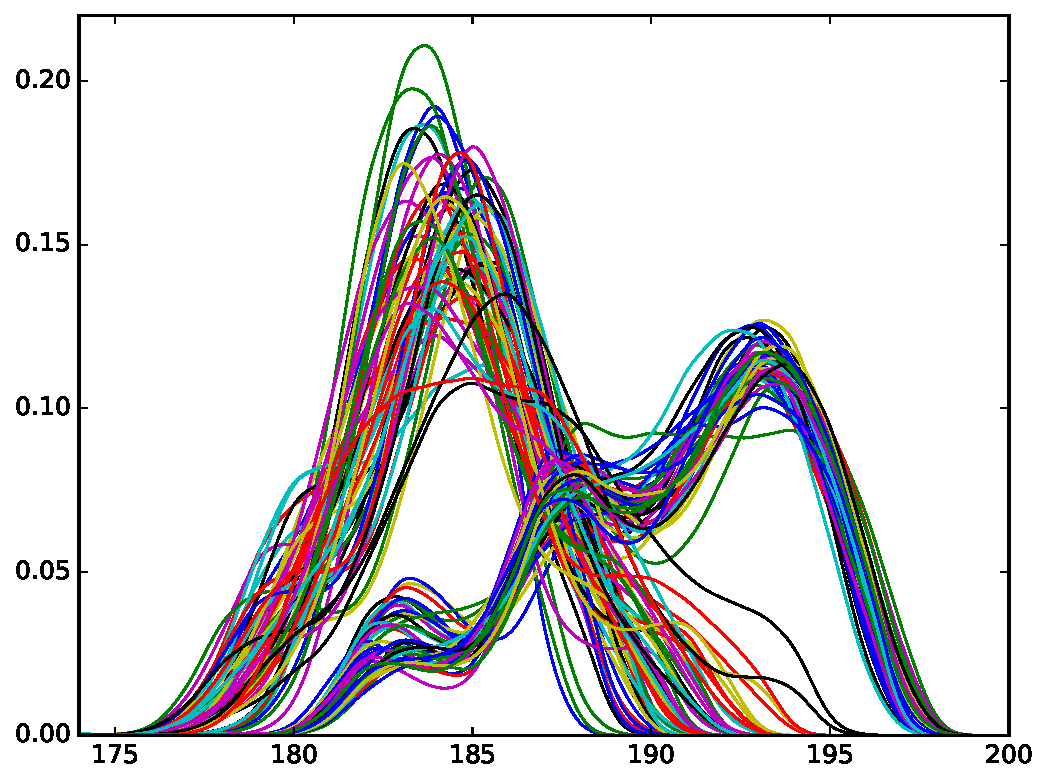
\includegraphics[width=\columnwidth]{figures/fig4/kde_pdf_sumindex}
\caption{Probability density functions (pdfs) from repeated trials of the
\lstinline|sumindex| benchmark. The pdfs form two distinct clusters, indicating
correlation across multiple trials.}
\label{fig:pdfsumindex}
\end{figure}

%%%%%%%%%%%%%%%%%%%%%%%%%%%%%%%%%%%%%%%%%%%%%%%%%%%%%%%%%%%%%%%%%%%%%%%%%%%%%%%%%%%%%%%%%%%%
\section{Limitations of our current approach}

We can't distinguish between a regression of the first kind and nonstationary jitter.

Another problem is that we see correlation in some benchmarks. Our bootstrap framework can't really deal with that.

We also don't deal with the multicore case. It is possible to extend our statistical
model to multiple noninteracting instruction streams, describing embarrassingly
parallel programs. However, we expect that interactions between streams, such as
resource contention or scheduling dependencies, will lead to entirely new
statistics which may not be adequately captured in our current model.
Related work:
Tsafrir et al. [18] describe “input shaking”, a technique for determining the sensitivity of their simulations of parallel systems. (Dan Tsafrir, Keren Ouaknine, and Dror G. Feitelson. Reducing performance evaluation sensitivity and variability by input shaking. In MASCOTS, 2007.)
Alameldeen and Wood[1] introduce variability in the latency of cache misses in order to alter thread-scheduling bias introduced by simulators that execute multi-threaded workloads. (Alaa R. Alameldeen and David A. Wood. Variability in architectural simulations of multi-threaded workloads. In IEEE HPCA,pages 7–18, 2003.)

%%%%%%%%%%%%%%%%%%%%%%%%%%%%%%%%%%%%%%%%%%%%%%%%%%%%%%%%%%%%%%%%%%%%%%%%%%%%%%%%%%%%%%%%%%%%

\section{Conclusion}

Our methodology can be applied in other comparisons of program performance
outside of regression testing, such as testing for performance differences under different compiler flags~\cite{Mytkowicz2009}.

\TODO{The conclusion goes here.}

%%%%%%%%%%%%%%%%%%%%%%%%%%%%%%%%%%%%%%%%%%%%%%%%%%%%%%%%%%%%%%%%%%%%%%%%%%%%%%%%%%%%%%%%%%%%

\section*{Acknowledgment}

We thank the many Julia developers, in particular Andreas Noack for many insightful discussions.

This work was supported by the Nanosoldier grant.\TODO{Get grant info}

\bibliography{biblio}
\bibliographystyle{IEEEtran}

% that's all folks
\end{document}
\grid
